%% LaTeX2e class for student theses
%% sections/main/5_design.tex
%%
%% Karlsruhe University of Applied Sciences
%% Faculty of  Computer Science and Business Information Systems
%%
%% --------------------------------------------------------
%% | Derived from sdqthesis by Erik Burger burger@kit.edu |
%% --------------------------------------------------------

\chapter{Design}
\label{ch:Design}

According to the collected requirements and use cases, the \acrshort{cs} reservation system has to fulfill, this chapter provides an approach covering the design process from the conceptualization of the required entities, the resulting workflows to the design of the endpoints utilizing the concepts of \acrshort{rest} described in \ref{ch:Fundamentals:sec:Data Exchange:ssec:REST}. 

\section{Entities}
\label{ch:Design:sec:Entities}

For representation of the resources defined in \ref{ch:Design:sec:Resources}, the following entities were created. 
For the selection of the required properties each entity owns, the standard protocols like \acrshort{ocpp} mentioned in \ref{ch:Fundamentals:sec:Electric Mobility:ssec:Relevant Standards:sssec:OCPP} are considered. 

\begin{figure}[!ht]
    \centering
    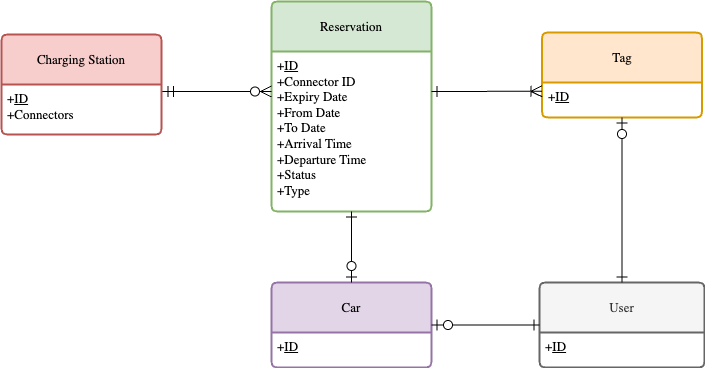
\includegraphics[scale=0.4]{resources/images/main/5_design/Entities.png}
    \caption{Entities and their relationships based on the provided scenario}
    \label{fig:entity-relationship-diagram}
\end{figure}

\section{Use Cases}
\label{ch:Design:sec:Use Cases}

To provide a basic feature set for the reservation system to work, the following use cases out of the chapter \ref{ch:Requirements Engineering} are selected. Based on this subset of features workflows are designed, the system has to implement for proper functionality.

Before implementation, the features are described and implemented using Flowchart diagrams with UML \cite{noauthor_welcome_nodate}.

\subsection{Create Reservation}
\label{ch:Design:sec:Use Cases:ssec:Create Reservation}

For creating a reservation the following steps are necessary.

\begin{figure}[!ht]
    \centering
    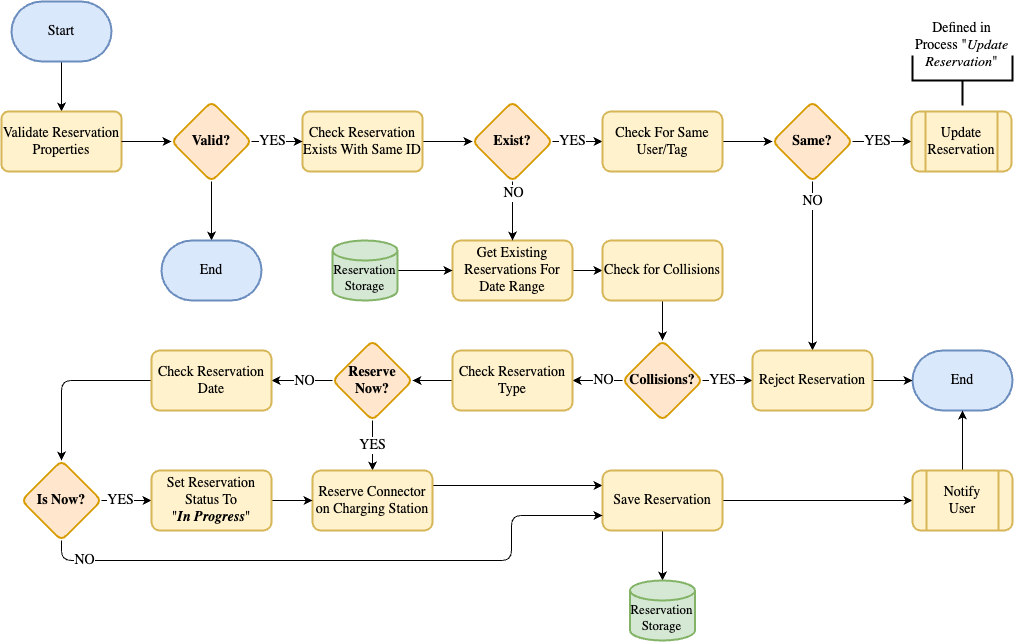
\includegraphics[scale=0.4]{resources/images/main/5_design/processes/ReservationCreate.png}
    \caption{Process flow and required steps for creating a reservation}
    \label{fig:create-reservation-flowchart}
\end{figure}

... including the design of the mockups for later implementation:

\begin{figure}
    \centering
     \begin{subfigure}[b]{0.6\textwidth}
         \centering
         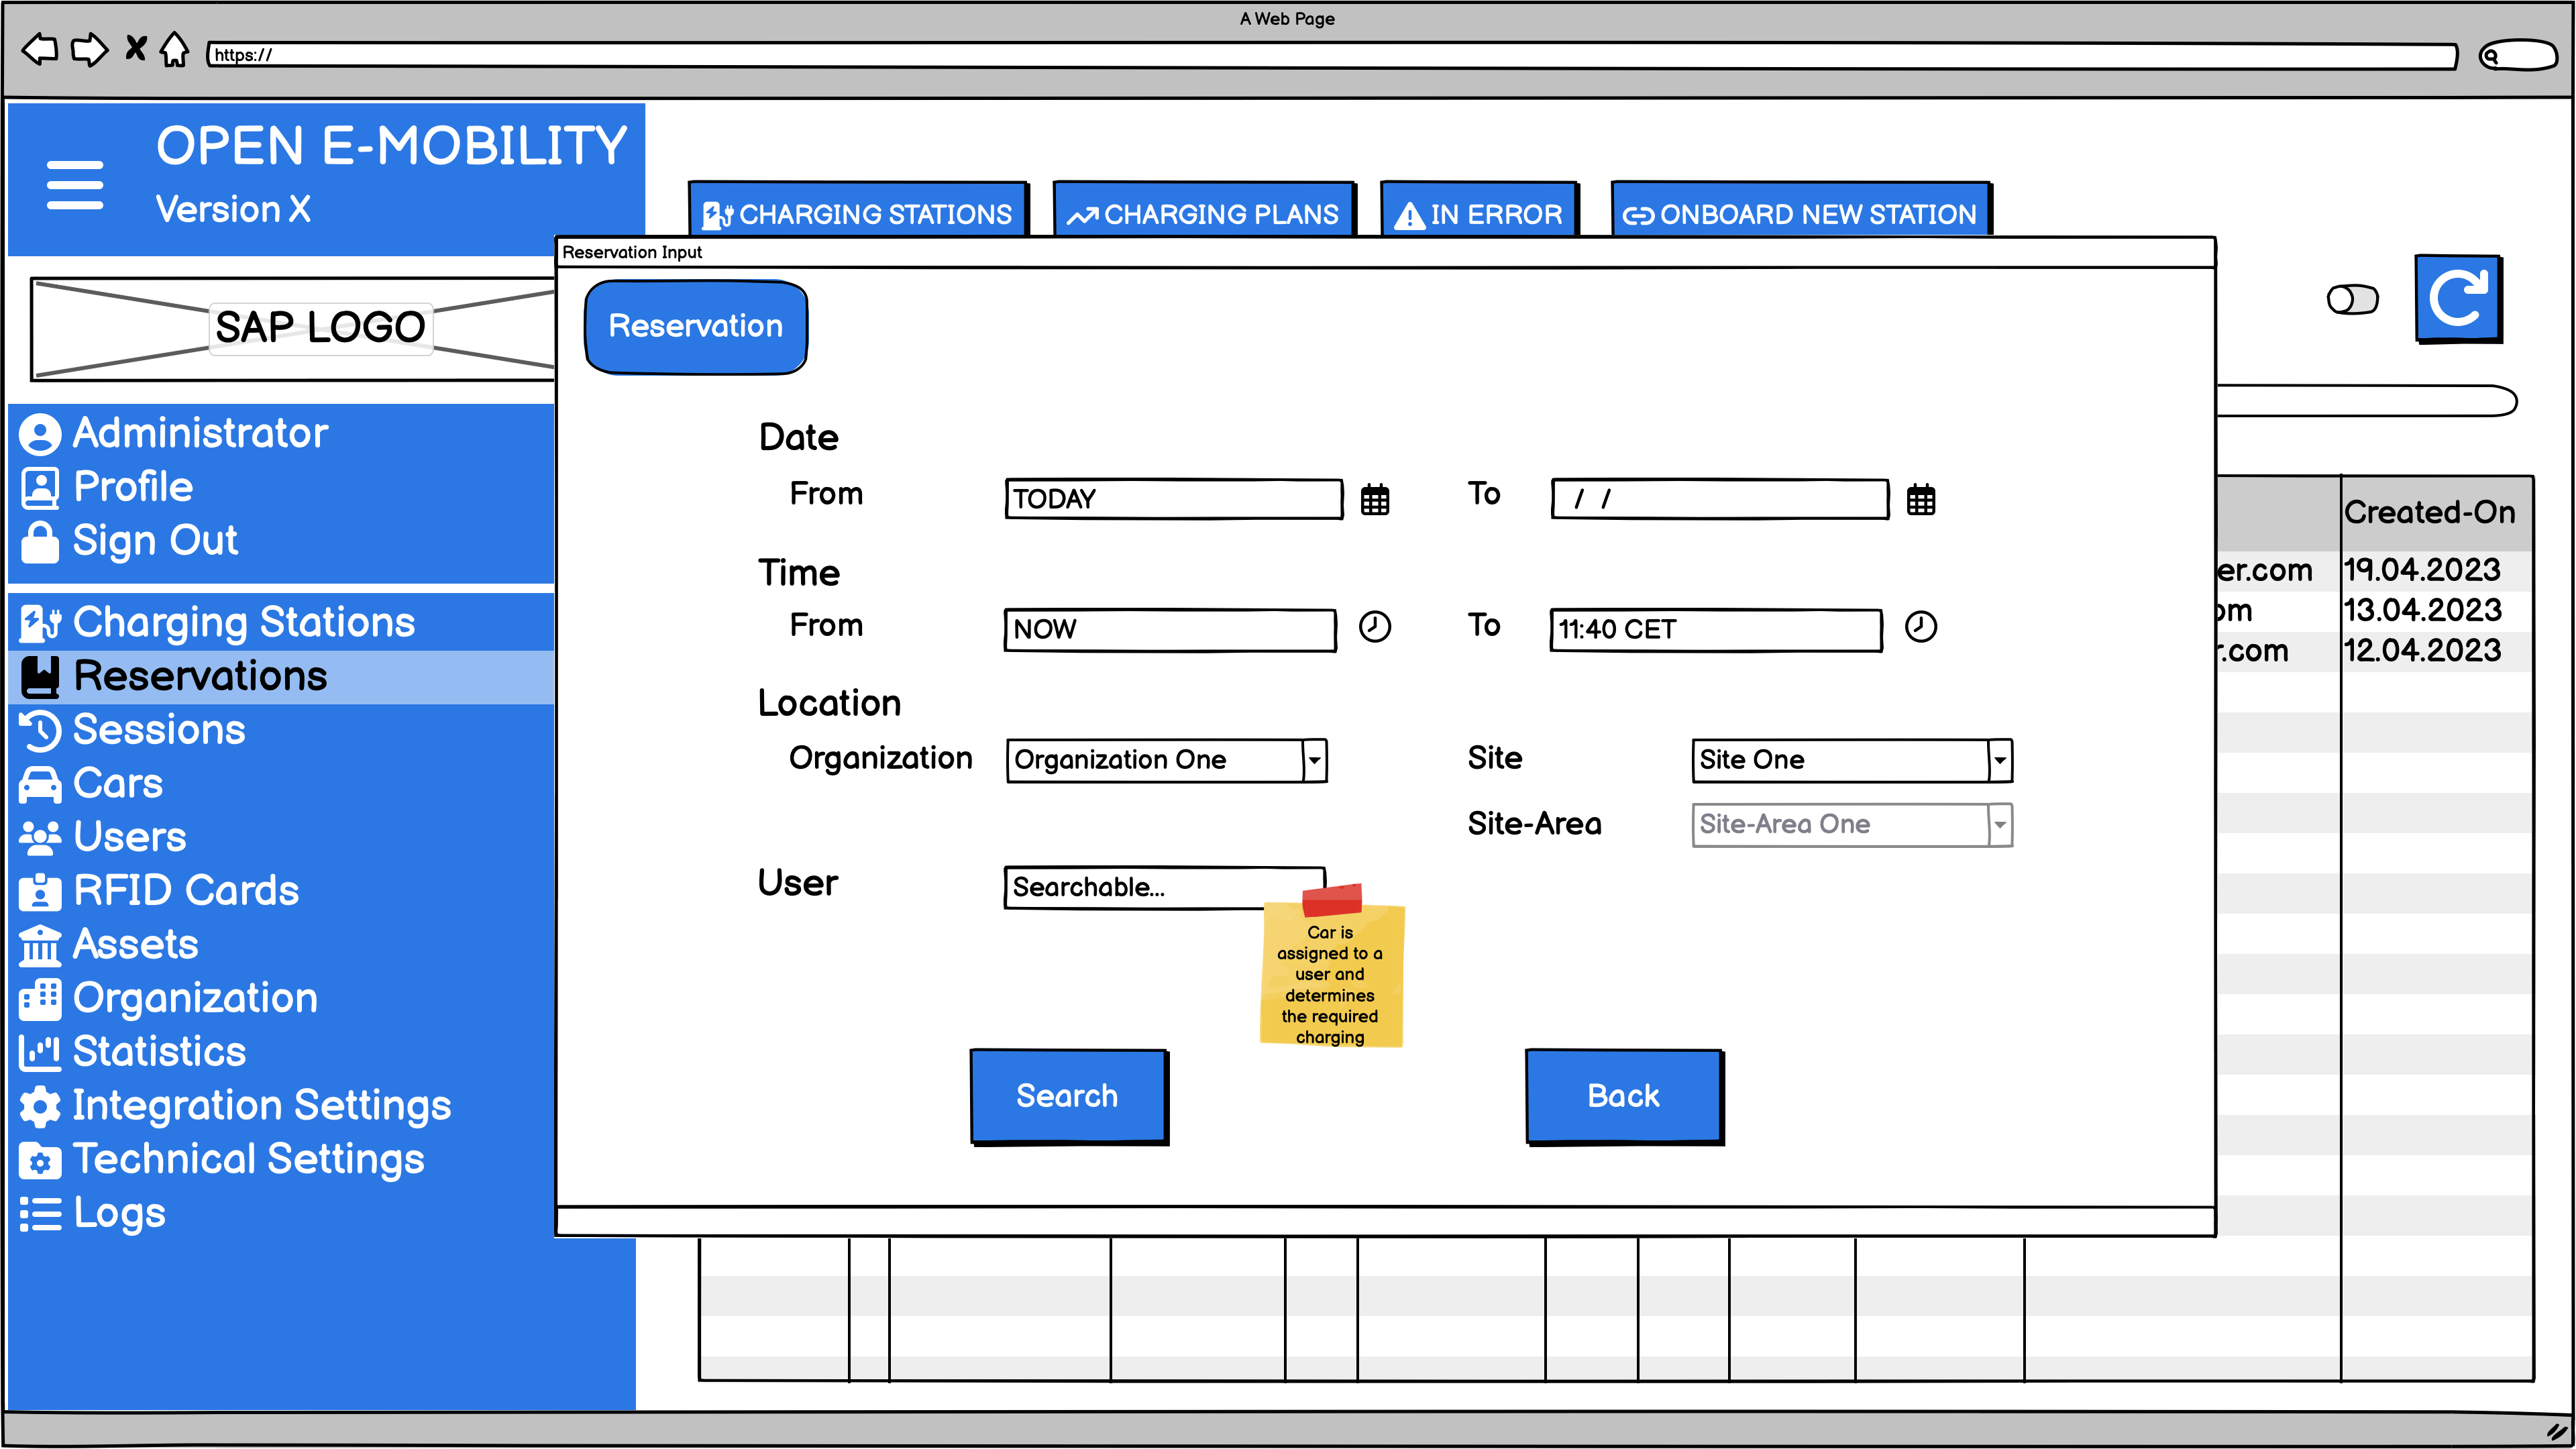
\includegraphics[width=\textwidth]{resources/images/main/5_design/mockups/create_reservation/web/1_Reservation_Create.png}
         \caption{Web Frontend}
         \label{fig:web-create-reservation}
    \end{subfigure}
     \hfill
     \begin{subfigure}[b]{0.3\textwidth}
         \centering
         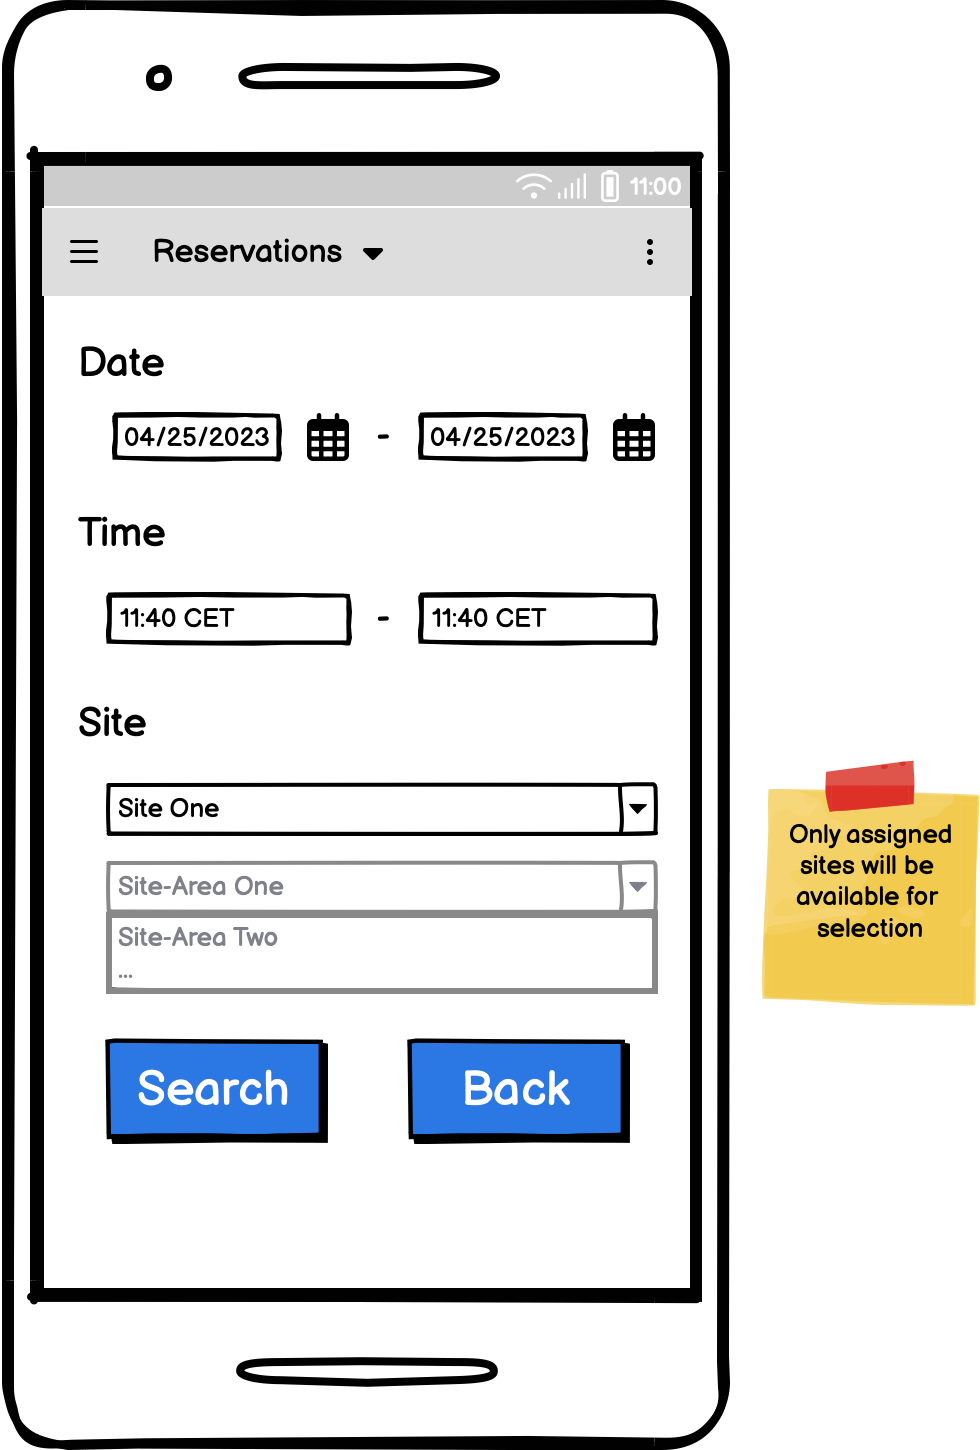
\includegraphics[width=\textwidth]{resources/images/main/5_design/mockups/create_reservation/mobile/2_Create_Reservation.png}
         \caption{Mobile}
         \label{fig:mobile-create-reservation}
    \end{subfigure}
    \caption{Comparison of mobile and web frontend regarding the creation of reservations}
    \label{fig:create-reservation-design}
\end{figure}

\subsection{Update Reservation}
\label{ch:Design:sec:Update Reservation}

For updating a reservation the following steps are necessary.

\begin{figure}[!ht]
    \centering
    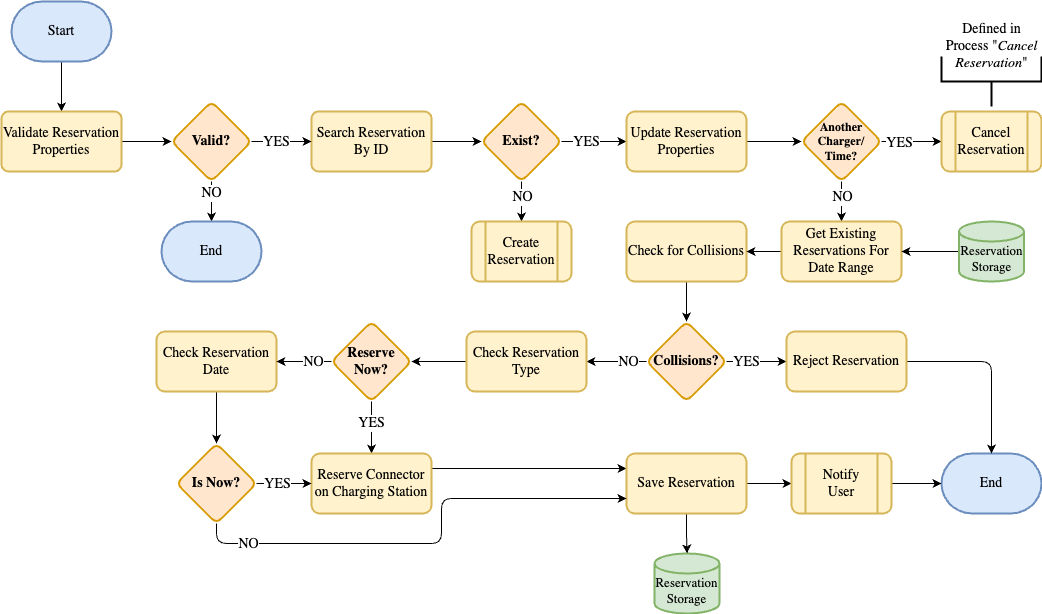
\includegraphics[scale=0.4]{resources/images/main/5_design/processes/ReservationUpdate.png}
    \caption{Process flow and required steps for updating a reservation}
    \label{fig:update-reservation-flowchart}
\end{figure}

\subsection{Delete Reservation}
\label{ch:Design:sec:Use Cases:ssec:Delete Reservation}

For deleting a reservation the following steps are necessary.

\begin{figure}[!ht]
    \centering
    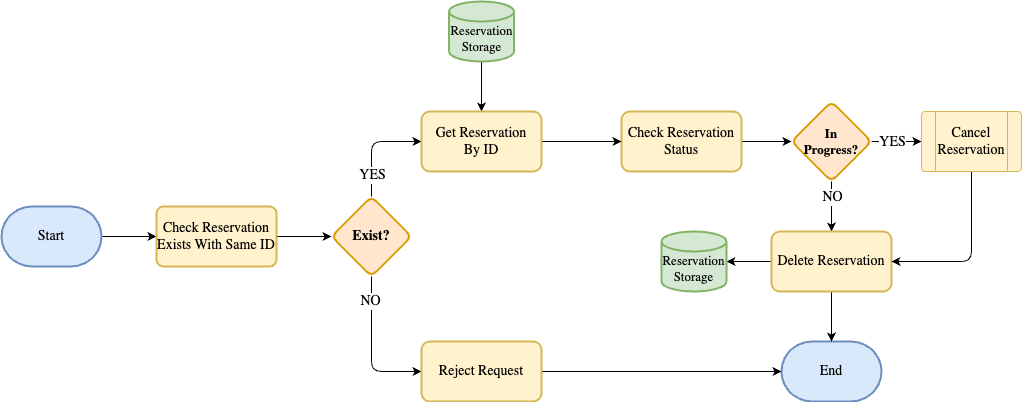
\includegraphics[scale=0.4]{resources/images/main/5_design/processes/ReservationDelete.png}
    \caption{Process flow and required steps for deleting a reservation}
    \label{fig:delete-reservation-flowchart}
\end{figure}

\subsection{Cancel Reservation}
\label{ch:Design:sec:Use Cases:ssec:Cancel Reservation}

\begin{figure}[!ht]
    \centering
    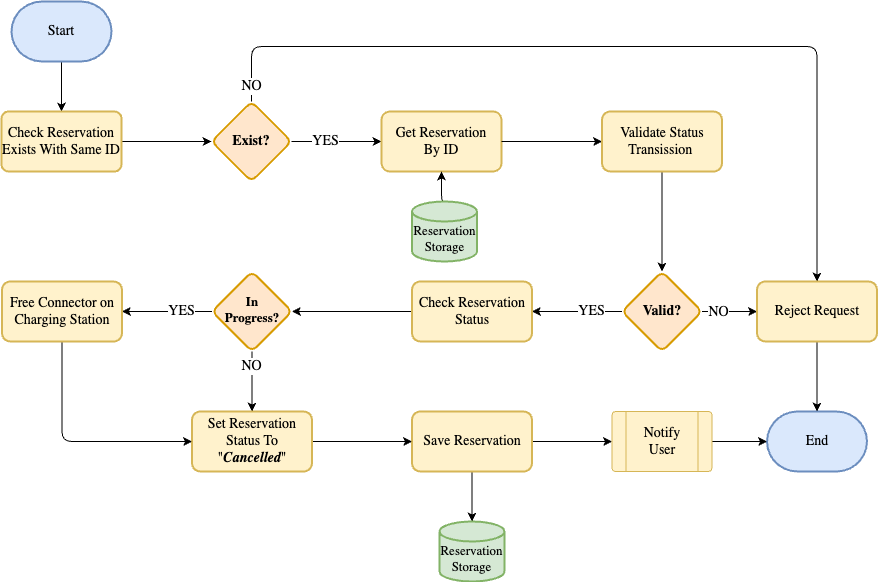
\includegraphics[scale=0.4]{resources/images/main/5_design/processes/ReservationCancel.png}
    \caption{Process flow and required steps for cancelling a reservation}
    \label{fig:cancel-reservation-flowchart}
\end{figure}

\subsection{Schedule Reservation}
\label{ch:Design:sec:Use Cases:ssec:Schedule Reservation}

\begin{figure}[!ht]
    \centering
    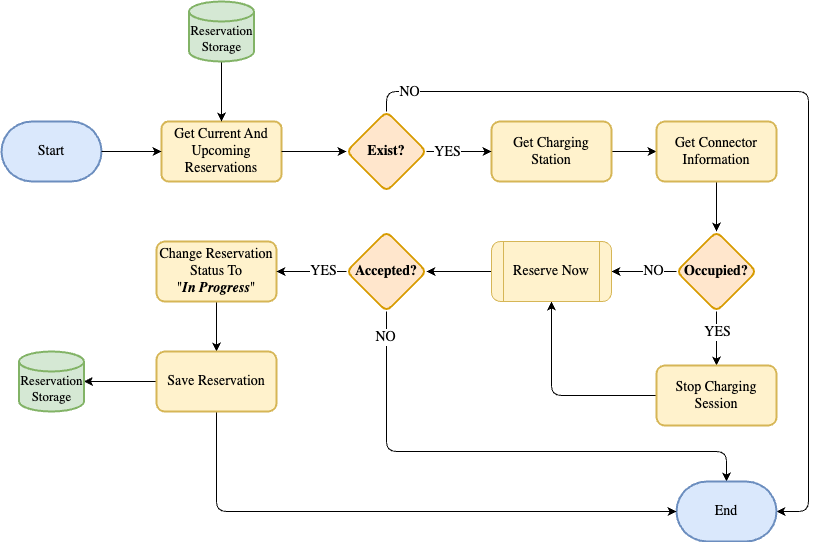
\includegraphics[scale=0.4]{resources/images/main/5_design/processes/scheduler/SynchronizeReservation.png}
    \caption{Process for scheduling upcoming reservation on the specified \acrshortpl{cs}}
    \label{fig:schedule-reservation-flowchart}
\end{figure}

\subsection{Expire Reservation}
\label{ch:Design:sec:Use Cases:ssec:Expire Reservation}

\begin{figure}[!ht]
    \centering
    
\includegraphics[scale=0.4]{resources/images/main/5_design/processes/scheduler/UpdateExpiredReservations.png}
    \caption{Process flow for reservations reaching their expiry date}
    \label{fig:expire-reservation-flowchart}
\end{figure}

\subsection{Free reserved connectors}
\label{ch:Design:sec:Use Cases:ssec:Free reserved connectors}

Afterwards the design of the process...

\begin{figure}[!ht]
    \centering
    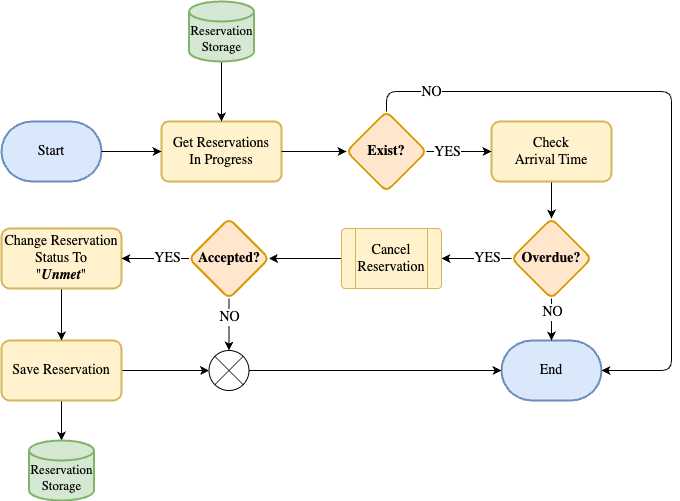
\includegraphics[scale=0.4]{resources/images/main/5_design/processes/scheduler/CancelUnmetReservation.png}
    \caption{Entities and their relationships based on the provided scenario}
    \label{fig:free-connector-flowchart}
\end{figure}

% Should include notifications descriptions in regards to 'Charging reservation service for electric vehicles using automatic notification'

% \section{Not Use Cases}
% \label{ch:Design:sec:Not Use Cases}

% \subsection{Smart Charging Integration}
% \label{ch:Design:sec:Not Use Cases:sec:Smart Charging}
